\documentclass[a4paper,10pt,twocolumn]{article}

\usepackage[font=small]{caption}
\usepackage{lipsum}
\usepackage{graphicx}
\usepackage{gensymb}
\usepackage{fancyhdr}
\pagestyle{empty}
\renewcommand{\headrulewidth}{0pt}
\renewcommand{\footrulewidth}{0pt}
\setlength\headheight{80.0pt}
\addtolength{\textheight}{-80.0pt}
\lhead{
\includegraphics[scale=0.085]{imagens/28.png}}

%Layout
\setlength\columnsep{0.8cm}
\setlength\topmargin{3.3cm}
\setlength\textheight{23.4cm}
\setlength\textwidth{7.5cm}
\usepackage[bottom=4.2cm]{geometry}

%Pacotes
\usepackage{amsthm,amssymb,amsmath}
\usepackage[brazil]{babel}
\usepackage[utf8]{inputenc}
\usepackage{amsfonts}
\usepackage{natbib}
\usepackage{titlesec}
\titlespacing*{\section}{0pt}{2pt}{2pt}
\usepackage{graphicx}
\usepackage{float}


%Fonte Arial
\renewcommand{\rmdefault}{phv}
\renewcommand{\sfdefault}{phv}
\usepackage{color}

\usepackage{geometry}
\geometry{
	a4paper,
	total={210mm,297mm},
	left=2.6cm,
	right=2.6cm,
	top=3.3cm,
	bottom=4.2cm
}

\begin{document}
	\pagenumbering{gobble}
	\title{\large{\vspace{-1cm}\textbf{Reconstrução de curvas por meio de características robustas em imagens}}}
	\author{\textbf{André Luís Mendes Fakhoury}\vspace{0.2cm}\\
		\textbf{Orientador: João E.S. Batista Neto}\vspace{0.2cm}\\
		Instituto de Ciências Matemáticas e de Computação, ICMC-USP\vspace{0.1cm}\\
		\normalsize{andrefakhoury@usp.br \quad }
		}
	
	\date{\null}
	\maketitle
	
	\thispagestyle{fancy}
	
	\section*{\hfil Objetivos}
	
	O objetivo deste projeto de pesquisa é extrair características robustas em $\mathbb{R}^2$ para reconstrução de curvas obtidas em imagens. Com isso, visa analisar algoritmos para o pré-processamento de imagens, extração de contorno de objetos, análise de pontos importantes de curvas e a respectiva reconstrução da curva original.
	
	\section*{\hfil Métodos e Procedimentos}
	As etapas de desenvolvimento do projeto podem ser visualizadas no diagrama da figura \ref{fig:diagrama}.
	\begin{figure}[ht!]
	\centering
	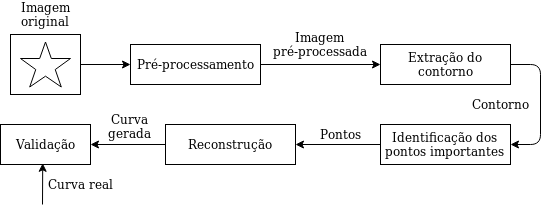
\includegraphics[width=0.84\linewidth]{imagens/diagrama.png}
	\caption{Diagrama de blocos de desenvolvimento.}
	\label{fig:diagrama}
	\end{figure}
	O pré-processamento visa a eliminação de pontos espúrios no contorno, de forma a permitir a extração de curvatura que melhor corresponda ao contorno original. A identificação dos pontos importantes é realizada a partir do cálculo da curvatura discreta do contorno. A reconstrução da curva baseia-se no método descrito por Sorkine \cite{sorkine} a partir de poucos pontos (âncoras) e informações de conectividade, utilizando uma discretização do operador de Laplace-Beltrami. A validação consiste em se calcular, quantitativamente, a distância euclidiana entre a curva original e a curva reconstruída.
	
	\section*{\hfil Resultados}
	
	A figura \ref{fig:leafs} ilustra a aplicação do método sobre uma folha para 30, 40 e 60 pontos. Quanto maior o número de pontos âncora, mais precisa é a reconstrução da forma original. O método também foi aplicado sobre imagens de faces humanas, curvas em $\mathbb{R}^3$ e malhas poligonais.
	

	\begin{figure}[ht!]
		\centering
		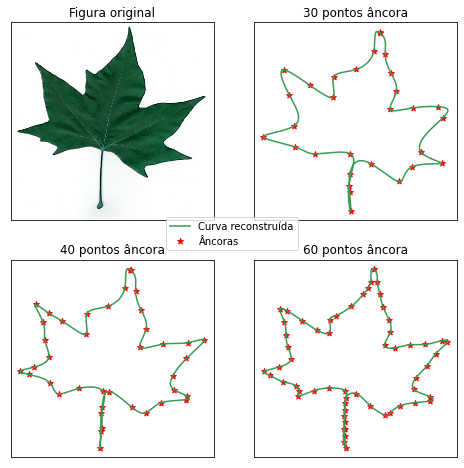
\includegraphics[width=0.81\linewidth]{imagens/leafs.png}
		\caption{Reconstrução em uma imagem de folha.}
		\label{fig:leafs}
	\end{figure}
	
	
	\section*{\hfil Conclusões}
	A utilização do operador discreto de Laplace-Beltrami permite uma boa reconstrução, se forem utilizados pontos âncora suficientes e escolhidos de maneira correta (por exempo, pela curvatura). Porém alguns detalhes da malha original podem se perder, pois não serão considerados pelo algoritmo.
	
	\bibliographystyle{unsrt}
	\renewcommand\refname{\hfil Referências Bibliográficas \hfil}
%\bibliography{artigo}
	\begin{center}
	\begin{thebibliography}{LLL}	
	\bibitem{sorkine}{SORKINE, O. Differential representations for mesh processing. \textit{Computer Graphics Forum}, European Association for Computer Graphics, v. 25, n. 4, p. 789–807, 2006.}
	\end{thebibliography}
	\end{center}
	
	\section*{\hfil Apoio}
	O projeto é financiado pela FAPESP (Fundação de Amparo à Pesquisa do Estado de São Paulo), nº 2020/07224-5, e também é parte do projeto temático FAPESP de nº 2019/07316-0.
	
	
\end{document}

